\newif\ifEnglish
\Englishfalse
\Englishtrue

\documentclass[unicode]{beamer}

\usepackage[orientation=portrait,size=a0,scale=1.1]{beamerposter}

\usetheme[footertext={JADH 2026 \textbullet\ September 11--13, 2026 \textbullet\ Kyushu University}]{SimplePoster}

\usefonttheme{professionalfonts}
\useinnertheme{rectangles}

\usepackage{version}
\usepackage{luatexja}
\usepackage{graphicx}
\usepackage{svg}
\usepackage{natbib}
\usepackage{float}
\renewcommand{\kanjifamilydefault}{\gtdefault}

\usepackage{caption}
\captionsetup{format=hang, labelfont=bf, labelsep=colon, font=small}
\setbeamertemplate{caption}[numbered]

\usepackage{array}
\usepackage{longtable}
\usepackage{colortab}
\usepackage{colortbl}
\usepackage{arydshln}
\usepackage{tcolorbox}
\usepackage{tikz}

\usebackgroundtemplate{%
  \begin{tikzpicture}[remember picture,overlay]
    \node[opacity=0.3,anchor=west,inner sep=0pt] at (current page.west) {%
      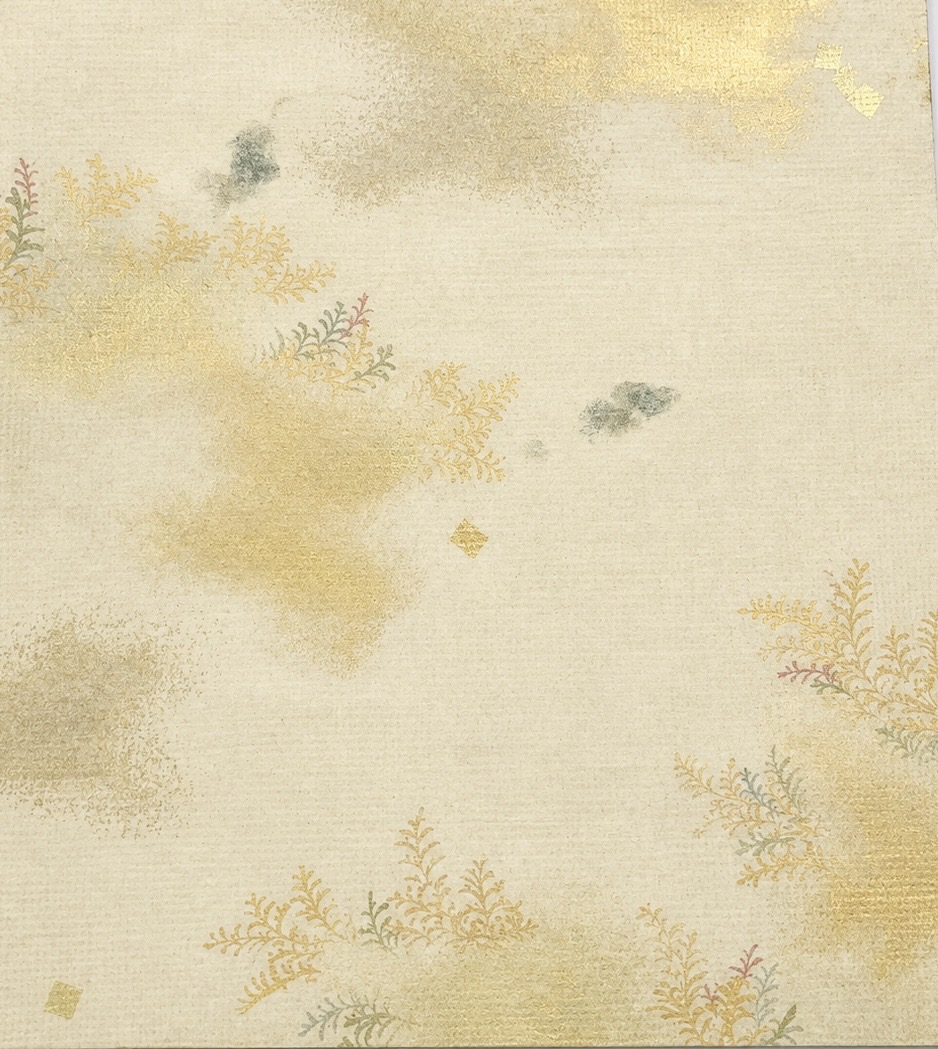
\includegraphics[height=\paperheight]{../images/poster-background2.jpg}%
    };
  \end{tikzpicture}%
}

\usepackage{fontspec}
\newfontfamily\emojifont{NotoColorEmoji}[
  Path=/nix/store/557hw66ma67d9csqbv7s8m593wzh3b01-noto-fonts-color-emoji-2.051/share/fonts/noto/,
  Extension=.ttf,
  Renderer=HarfBuzz
]

\title{Kugire Data Curation for the Kokinwakashu TEI/XML Data}

\author{Xudong Chen\inst{{\emojifont 🐻}} \and Bor Hodošček\inst{{\emojifont 🐊}} \and Hilofumi Yamamoto\inst{{\emojifont 🐦}}}
\institute{\inst{{\emojifont 🐻}}Waseda University \quad \inst{{\emojifont 🐊}}The University of Osaka \quad \inst{{\emojifont 🐦}}Institute of Science Tokyo}


\newsavebox{\topfigbox}
\newsavebox{\inputdatabox}
\newlength{\topfigheight}
\newlength{\bodycolumnheight}
\newlength{\subcolwidth}
\newlength{\inputdataheight}
\newlength{\nestedheight}
\newlength{\topfigvfillreserve}
\newlength{\postercolwidth}
\newlength{\postergap}
\newlength{\leftgroupwidth}

\begin{document}
\begin{frame}[t]

\setlength{\postergap}{0.02\textwidth}
\setlength{\postercolwidth}{\dimexpr(\textwidth-2\postergap)/3\relax}
\setlength{\leftgroupwidth}{\dimexpr2\postercolwidth+\postergap\relax}

\savebox{\topfigbox}{\begin{minipage}[t]{\leftgroupwidth}\begin{figure}[H]\centering
\includesvg[inkscapelatex=false, inkscapearea=page, width=0.95\textwidth]{../images/fig-sarumaru-triptych}
\setcounter{figure}{0}
\caption{An example for the kugire-based interpretive diversity of poem no.\,215}
\end{figure}

{\large
\begin{itemize}
\item Kugire has interpretive diversity and reflects discourse-level interpretive diversity
\item Lack of structured kugire data
\item Kugire data $\rightarrow$ Ten translators + morphological rules inconsistence
\end{itemize}
}
\end{minipage}}
\setlength{\topfigheight}{\ht\topfigbox}
\addtolength{\topfigheight}{\dp\topfigbox}
\setlength{\bodycolumnheight}{\dimexpr\textheight-2\baselineskip\relax}
\setlength{\topfigvfillreserve}{0.015\bodycolumnheight}
\setlength{\nestedheight}{\bodycolumnheight}
\addtolength{\nestedheight}{-\topfigheight}
\addtolength{\nestedheight}{-\topfigvfillreserve}

  \noindent
  \begin{minipage}[t][\bodycolumnheight][t]{\leftgroupwidth}
      \setlength{\subcolwidth}{\postercolwidth}%
      \savebox{\inputdatabox}{\begin{minipage}[t]{\subcolwidth}\begin{block}{Input data}

\begin{figure}[H]\centering
\includesvg[inkscapelatex=false, width=0.9\textwidth]{../images/fig3-resource-relationship}
\setcounter{figure}{4}
\caption{Relationships among the project's data sources and tools: TEI/XML merge,
vocabulary datasets, search and network-visualization tools, translation corpus.}
\end{figure}

\begin{enumerate}
\item \textbf{Base TEI/XML}: the Kokinwakashu text, five-ku segmentation, author
  information, textual variants, commentary, and other existing TEI markup
\item \textbf{Vocabulary and morphological information}: the Hachidaishu vocabulary
  list and part-of-speech data; used to infer kugire candidates from inflection
  forms, sentence-final particles, binding particles, etc.
\item \textbf{Modern Japanese translation}: the modern Japanese gloss in Kaneko
  Motoomi's \textit{Kokinwakashu Hy\=osh\=aku}; used to observe how 20th-century
  commentators construed the waka as modern Japanese discourse
\end{enumerate}
\end{block}
\end{minipage}}%
      \setlength{\inputdataheight}{\ht\inputdatabox}%
      \addtolength{\inputdataheight}{\dp\inputdatabox}%
      \usebox{\topfigbox}%
      \vfill
      \par\nointerlineskip
      \noindent
      \begin{minipage}[t][\nestedheight][s]{\postercolwidth}
          \begin{minipage}[t][\inputdataheight][s]{\linewidth}
          \begin{block}{What Does This Work Do?}
Classical Japanese poetry, a.k.a.\ waka, consists of 5/7/5/7/7-syllable phrases.
Kugire are grammatical/semantic pauses within the phrases.

Kugire (句切れ) are phrase/clause breaks within waka poems. We try to describe
kugire with structured data and provide multiple sources of evidence, covering:
\begin{enumerate}
\item Annotating \textbf{non-visible} interpretive elements in structured data
\item How annotation preserves the source and reliability of information
\item Interpretive diversity at the discourse level
\end{enumerate}
\end{block}

          \vfill
          \begin{block}{Why Kugire?}
\begin{itemize}
\item We perform analysis on interpretive diversity for visible lexical elements in waka
\item Analysis on invisible discourse-level elements was not performed yet
\item Kugire shows discourse-level interpretability
\end{itemize}

\vspace{-\dimexpr\parskip+\topsep+\partopsep+\parsep+.65\baselineskip\relax}
{\setlength{\intextsep}{0pt}%
\setlength{\textfloatsep}{0pt}%
\setlength{\floatsep}{0pt}%
\begin{figure}[H]
\begin{minipage}[t]{0.55\linewidth}
  \centering
  \includesvg[inkscapelatex=false, width=0.9\textwidth]{../images/fig-miru}
  \setcounter{figure}{1}
  \caption{Interpretive diversity of the predicate of \textit{miru} (see)}
\end{minipage}%
\hfill
\begin{minipage}[t]{0.42\linewidth}
  \centering
  \includesvg[inkscapelatex=false, width=0.9\textwidth]{../images/fig-ominaeshi}
  \setcounter{figure}{2}
  \caption{Interpretive diversity of lexical space \textit{ominaeshi} (``maidenflower'')}
\end{minipage}
\end{figure}
}
\end{block}

          \end{minipage}
          \vfill
          \begin{block}{Output data}

The output file is \texttt{kokin-kugire.xml}. Each kugire candidate is appended as
a \texttt{<k>} element inside the corresponding \texttt{<l>}, keeping at least:
\begin{itemize}
\item \texttt{@n}: which segment the kugire falls after
\item \texttt{@source}: the judgment source, e.g.\ \texttt{morph} or \texttt{kaneko}
\item \texttt{@cert}: the certainty given by the grammatical rule (\texttt{high}/\texttt{mid}/\texttt{low})
\end{itemize}

A single poem can retain multiple \texttt{<k>} elements --- this preserves both the
grammatically visible break point and the interpretive break point evidenced in
translation side by side.

\texttt{<k>} is a project-internal tag pending a decision on the target TEI encoding.
A future revision will replace it with \texttt{<anchor>} and \texttt{<standOff>}:

\definecolor{xmlgray}{HTML}{888888}
\definecolor{xmltag}{HTML}{0055AA}
\definecolor{xmlattr}{HTML}{AA3300}
\definecolor{xmlval}{HTML}{007700}

\begin{figure}[H]\centering
\begin{tcolorbox}[colback=black!2, colframe=black!15, boxrule=0.5pt, arc=2pt,
  width=0.9\textwidth, left=8pt, right=8pt, top=6pt, bottom=6pt]
\ttfamily\small
\textcolor{xmlgray}{<}\textcolor{xmltag}{seg}\textcolor{xmlgray}{>}年の内に\textcolor{xmlgray}{</}\textcolor{xmltag}{seg}\textcolor{xmlgray}{>}\\[2pt]
\textcolor{xmlgray}{<}\textcolor{xmltag}{anchor} \textcolor{xmlattr}{xml:id}\textcolor{xmlgray}{=}"\textcolor{xmlval}{n1\_break\_after\_2}"\textcolor{xmlgray}{/>}\\[2pt]
\textcolor{xmlgray}{<}\textcolor{xmltag}{seg}\textcolor{xmlgray}{>}春はきにけり\textcolor{xmlgray}{</}\textcolor{xmltag}{seg}\textcolor{xmlgray}{>}\\[8pt]
\textcolor{xmlgray}{<}\textcolor{xmltag}{standOff}\textcolor{xmlgray}{>}\\[2pt]
\hspace*{1.5em}\textcolor{xmlgray}{<}\textcolor{xmltag}{interpGrp} \textcolor{xmlattr}{type}\textcolor{xmlgray}{=}"\textcolor{xmlval}{kugire}"\textcolor{xmlgray}{>}\\[2pt]
\hspace*{3em}\textcolor{xmlgray}{<}\textcolor{xmltag}{interp} \textcolor{xmlattr}{target}\textcolor{xmlgray}{=}"\textcolor{xmlval}{\#n1\_break\_after\_2}"\\[2pt]
\hspace*{5em}\textcolor{xmlattr}{source}\textcolor{xmlgray}{=}"\textcolor{xmlval}{\#morph}" \textcolor{xmlattr}{cert}\textcolor{xmlgray}{=}"\textcolor{xmlval}{high}"\textcolor{xmlgray}{/>}\\[2pt]
\hspace*{3em}\textcolor{xmlgray}{<}\textcolor{xmltag}{interp} \textcolor{xmlattr}{target}\textcolor{xmlgray}{=}"\textcolor{xmlval}{\#n1\_break\_after\_2}"\\[2pt]
\hspace*{5em}\textcolor{xmlattr}{source}\textcolor{xmlgray}{=}"\textcolor{xmlval}{\#kaneko}"\textcolor{xmlgray}{/>}\\[2pt]
\hspace*{1.5em}\textcolor{xmlgray}{</}\textcolor{xmltag}{interpGrp}\textcolor{xmlgray}{>}\\[2pt]
\textcolor{xmlgray}{</}\textcolor{xmltag}{standOff}\textcolor{xmlgray}{>}
\end{tcolorbox}
\setcounter{figure}{3}
\caption{TEI encoding scheme expressing kugire annotation using \texttt{<anchor>}
and \texttt{<standOff>}. Break position, judgment source, and certainty are recorded
separately, so a single poem can retain multiple interpretations.}
\end{figure}
\end{block}

      \end{minipage}\hspace{\postergap}%
      \begin{minipage}[t][\nestedheight][s]{\postercolwidth}
          \usebox{\inputdatabox}
          \vfill
          \begin{block}{Translation-Based Annotation}
Uses Kaneko's modern Japanese gloss as interpretive evidence. A locally run LLM
(\texttt{qwen2.5} / Ollama) first aligns the poem's five segments with the modern
Japanese translation, then finds sentence- or discourse-level breaks in the
translation, and finally maps them back onto segment positions in the original
poem. This method emphasizes ``the places read as broken in interpretive
practice.''

Human review and TEI output: automatically generated candidates are first
written to a per-poem cache file, then checked, added to, or corrected by a
human reviewer. The confirmed result is written back to TEI/XML, so the data
stays traceable to the evidence behind each kugire judgment.

\begin{figure}[H]\centering
\includesvg[inkscapelatex=false, width=0.9\textwidth]{../images/fig-annotation-pipeline-tikz}
\setcounter{figure}{5}
\caption{Annotation pipeline from poem and translation, through LLM
suggestion and human review, to TEI/XML output.}
\end{figure}
\end{block}

      \end{minipage}%
  \end{minipage}\hspace{\postergap}%
  \begin{minipage}[t][\bodycolumnheight][s]{\postercolwidth}
      \begin{block}{Morphology-Based Kugire Annotation}
Searches the morphological data for positions that may form a kugire. Conclusive
forms, imperative forms, realis forms, sentence-final particles, etc.\ serve as
strong candidates; binding particles, kakari-musubi, taigen-dome, etc.\ serve as
moderate-to-weak candidates. This method emphasizes ``grammatically observable
break points.''

\vspace{1.0ex}

\begin{figure}[H]\centering
\includesvg[inkscapelatex=false, width=0.9\textwidth]{../images/example}
\setcounter{figure}{6}
\caption{Three classes of kugire candidates derived from morphological information:
strong, moderate, and weak candidates. This figure illustrates that the rule-based
method does not give a single answer, but candidate interpretations with certainty
levels.}
\end{figure}
\end{block}

      \vfill
      \begin{block}{WIP Results}
\begin{itemize}
\item Broadly similar readings show high agreement, but divergent interpretations always remain
\end{itemize}

\vspace{1.0ex}

\begin{figure}[H]\centering
\includesvg[inkscapelatex=false, width=0.85\textwidth]{../images/fig-translator-alpha-distribution}
\setcounter{figure}{7}
\caption{Distribution of agreement among ten translators over four possible
kugire positions (Krippendorff's alpha computed per poem).}
\end{figure}

\vspace{1.0ex}

\begin{figure}[H]\centering
\includesvg[inkscapelatex=false, width=0.85\textwidth]{../images/fig-cumulative-11-judgement-agreement}
\setcounter{figure}{8}
\caption{Cumulative inter-judge agreement: number and percentage of poems (out
of 1000) where at least N of the 11 judgment sources agree on the kugire
position, for N = 6 through 11.}
\end{figure}
\end{block}

  \end{minipage}

\end{frame}
\end{document}
